\begin{yl}{5}{Hinded}{hinded}{1 sek / 5 sek}{60 punkti}
  \emph{Idee ja teostus: Targo Tennisberg, lahenduse selgitus: Tähvend Uustalu}

  Lahutame igast lahtrist arvu 50. Nüüd taandub ülesanne kujule
  \begin{quote}
    On antud ruudustik $A$. Igasse lahtrisse on kirjutatud üks arv.
    Leia ruudustikus selline ristkülik, mille summa on kõikide ristkülikute seas vähim võimalik.
  \end{quote}

  Selle ülesande lahendamiseks on kõigepealt hea teada, kuidas kiiresti
  arvutada alamristkülikute summasid. Teeme seda nn osasummade meetodi
  abil (ingl k. \textit{prefix sums}): arvutame välja teise maatriksi $B$ nii, et
  $B[i][j]$ on maatriksi $A$ kõigi nende lahtrite summa, mis jäävad lahtrist
  $(i, j)$ vasakule ja üles (ehk nende lahtrite, mille rea number on ülimalt
  $i$ ja veeru number ülimalt $j$).

  \begin{figure}[h]
    \centering
    \subfloat[{$B[i][j]$} definitsioon]{
      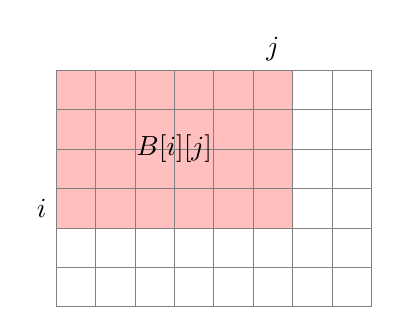
\begin{tikzpicture}[scale=0.5]
        \fill[pink] (0, 2) rectangle (6, 6);
        \draw[gray, very thin] (0, 0) grid (8, 6);
        \draw (0, 2.5) node[left]{$i$};
        \draw (5.5, 6) node[above]{$j$};
        \draw (3, 4) node{$B[i][j]$};
      \end{tikzpicture}
    }
    \qquad
    \subfloat[Valemi (\ref{pie}) piirkonnad]{
      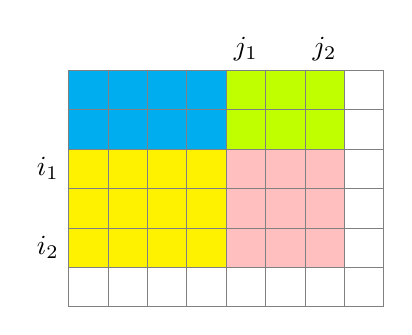
\begin{tikzpicture}[scale=0.5]
        \fill[cyan] (0, 4) rectangle (4, 6);
        \fill[lime] (4, 4) rectangle (7, 6);
        \fill[yellow] (0, 1) rectangle (4, 4);
        \fill[pink] (4, 1) rectangle (7, 4);
        \draw[gray, very thin] (0, 0) grid (8, 6);
        \draw (0, 3.5) node[left]{$i_1$};
        \draw (0, 1.5) node[left]{$i_2$};
        \draw (4.5, 6) node[above]{$j_1$};
        \draw (6.5, 6) node[above]{$j_2$};
      \end{tikzpicture}
      \label{piefig}
    }
    \caption{Osasummad ja nende kasutamine}
  \end{figure}

  Nüüd on ristküliku $A[i_1 \ldots i_2][j_1 \ldots j_2]$ summa leitav valemiga
  \begin{equation} \label{pie}
    B[i_2][j_2] - B[i_1 - 1][j_2] - B[i_2][j_1 - 1] + B[i_1 - 1][j_1 - 1].
  \end{equation}
  Tõepoolest:
  \begin{xitem}
  \item Lahter, mis asub ristküliku sees (joonisel \ref{piefig} punane piirkond), on
    esindatud ainult liidetavas $B[i_2][j_2]$.
  \item Lahter, mille rea number jääb $i_1$ ja $i_2$ vahele,
    kuid veeru number on väikesem
    kui $j_1$ (joonisel kollane piirkond), on esindatud liidetavates $B[i_2][j_2]$ ja
    $B[i_2][j_1 - 1]$. Nende märgid
    on valemis (\ref{pie}) vastupidised, seega need lahtrid summasse ei panusta.
  \item Lahter, mille veeru number jääb $j_1$ ja $j_2$ vahele,
    kuid rea number on väikesem
    kui $i_1$ (joonisel roheline piirkond), on esindatud liidetavates
    $B[i_2][j_2]$ ja $B[i_1 - 1][j_2]$. Nende märgid
    on valemis (\ref{pie}) vastupidised, seega need lahtrid summasse ei panusta.
  \item Lahter, mille rea number on väikesem kui $i_1$ ja veeru number väikesem kui $j_1$
    (joonisel sinine piirkond)
    on esindatud kõigis neljas liidetavas. Et kahel liidetaval on valemis (\ref{pie})
    plussmärk ja kahel miinusmärk, siis ka need lahtrid summasse ei panusta.
  \item Ülejäänud lahtrid ei panusta ühtegi liidetavasse.
  \end{xitem}

  Teisisõnu, kui valemis (\ref{pie}) kõik $B$-d $A$-de summana lahti kirjutada, siis
  taanduvad välja kõik liidetavad, välja arvatud need, mis on ristküliku $A[i_1 \ldots i_2][j_1 \ldots j_2]$ sees.
  Niisiis, kui meil on selline maatriks $B$ välja arvutatud, saame mistahes
  ristküliku elementide summa arvutada konstantse ($O(1)$) ajaga.

  \clearpage
  Maatriksi $B$ saab välja arvutada alloleva pseudokoodi abil:
\begin{lstlisting}[language=C++]
// B on (n + 1) x (n + 1) maatriks, alguses täidetud nullidega
// eeldame, et A elemendid on indekseeritud A[1..n][1..n]
for (int i = 1; i <= n; i++)
  for (int j = 1; j <= n; j++)
    B[i][j] = B[i][j - 1] + A[i][j];

for (int i = 1; i <= n; i++)
  for (int j = 1; j <= n; j++)
    B[i][j] += B[i - 1][j];
\end{lstlisting}
  Veendume selle korrektsuses.

  \begin{xenum}
  \item Hetkel, kui omistame \lstinline[language=C++]|B[i][j] = B[i][j - 1] + A[i][j]|, on (joonis \ref{reasummad})
    $B[i][j - 1]$ ristküliku $A[i][1 \ldots j - 1]$ summa. Seega
    $B[i][j - 1] + A[i][j]$ on ristküliku $A[i][1 \ldots j]$ summa.
  \item Hetkel, kui omistame \lstinline[language=C++]|B[i][j] += B[i - 1][j]|, on (joonis \ref{veerusummad})
    $B[i][j]$ ristküliku $A[i][1 \ldots j]$ summa, $B[i - 1][j]$ aga
    juba $A[1 \ldots i - 1][1 \ldots j]$ summa. Seega pärast tehte tegemist
    on $B[i][j]$ ristküliku $A[1 \ldots i][1 \ldots j]$ summa.
  \end{xenum}

  \begin{figure}[h]
    \centering
    \subfloat[Esimene tsükkel]{
      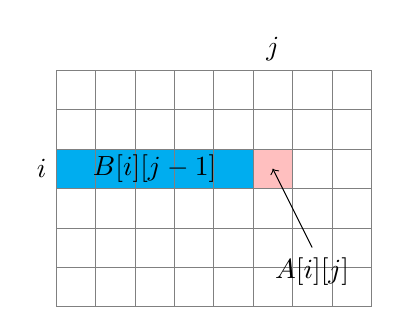
\begin{tikzpicture}[scale=0.5]
        \fill[cyan] (0, 3) rectangle (5, 4);
        \fill[pink] (5, 3) rectangle (6, 4);
        \draw[gray, very thin] (0, 0) grid (8, 6);
        \draw (0, 3.5) node[left]{$i$};
        \draw (5.5, 6) node[above]{$j$};
        \draw (2.5, 3.5) node{$B[i][j-1]$};
        \draw[->] (6.5, 1.5) node[below]{$A[i][j]$} -- (5.5, 3.5);
      \end{tikzpicture}
      \label{reasummad}
    }
    \qquad
    \subfloat[Teine tsükkel]{
      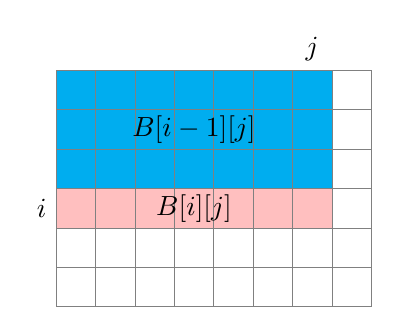
\begin{tikzpicture}[scale=0.5]
        \fill[cyan] (0, 3) rectangle (7, 6);
        \fill[pink] (0, 2) rectangle (7, 3);
        \draw[gray, very thin] (0, 0) grid (8, 6);
        \draw (0, 2.5) node[left]{$i$};
        \draw (6.5, 6) node[above]{$j$};
        \draw (3.5, 4.5) node{$B[i - 1][j]$};
        \draw (3.5, 2.5) node{$B[i][j]$};
      \end{tikzpicture}
      \label{veerusummad}
    }
    \caption{Osasummade arvutamine}
  \end{figure}

  Nii on võimalik maatriks $B$ arvutada välja $O(n^2)$ ajaga. Pärast välja arvutamist
  saab igale päringule vastata $O(1)$ ajaga.
  See annab meile ka automaatselt teise alamülesande lahenduse: käime läbi kõik
  nelikud $i_1, i_2, j_1, j_2$, arvutame valemi (\ref{pie}) abil välja iga ristküliku
  $A[i_1 \ldots i_2][j_1 \ldots j_2]$ summa ja võtame nendest summadest miinimumi.

  Saab aga ka paremini. Oletame, et oleme otsustanud $i_1, i_2$ ja $j_2$ väärtused.
  Peame leidma sellise $j_1 \le j_2$, mis minimeerib summat
  \[ B[i_2][j_2] - B[i_1 - 1][j_2] - B[i_2][j_1 - 1] + B[i_1 - 1][j_1 - 1]. \]
  Liidetavad $B[i_2][j_2]$ ja $-B[i_1 - 1][j_2]$ ei sõltu $j_1$ väärtusest. Seega
  võime sama hästi otsida sellist $j_1 \le j_2$, mis minimeerib summat
  \[ - B[i_2][j_1 - 1] + B[i_1 - 1][j_1 - 1]. \]
  See summa aga ei sõltu jälle kuidagi $j_2$ väärtusest. See viib meid täislahenduseni.
  Käime läbi kõik $i_1$ ja $i_2$ paarid. Iga paari kohta käime läbi kõik $j$-d kasvavas
  järjestuses. Iga $j$ korral jätame meelde $-B[i_2][j-1] + B[i_1][j-1]$ väärtuse.
  Seejärel valime juba meelde jäetud väärtuste seast vähima ja liidame sellele
  $B[i_2][j] - B[i_1 - 1][j]$:

  \clearpage
\begin{lstlisting}[language=C++]
int ans = INF;
for (int i1 = 1; i1 <= n; i1++) {
  for (int i2 = i1; i2 <= n; i2++) {
    int best = INF;
    for (int j = 1; j <= n; j++) {
      best = min(best, -B[i2][j - 1] + B[i1 - 1][j - 1];
      ans = min(ans, B[i2][j] - B[i1 - 1][j] + best);
    }
  }
}
\end{lstlisting}
\end{yl}
